\chapter{Participatory Design}
Autism as previously described comes with a vast array of difficulties, some of which may be too complex or time consuming to convey(such as social difficulties). It was consequently important to select the most salient aspects of Autism and the participatory design was conducted to facilitate these choices and the design of the prototype. 

\section{LAER Lab}
An initial consultation was held with Learning and Adaptive Environments Research(LAER) Lab which aims to "bring together academics and students interested in technologies designed or applied with the goal of furthering education". In attendance were several members(I have little idea of who these were or how to describe them...you, Alyssa...) as well as two other students whom were also creating software projects related autism. An overview of the simulator was given in addition to goals and suggestions(see appendix for notes on what was given). Children are exposed to a plethora of different environment on a day to day basis(school, work, parks, etc), however, the most common location for a child is the home and thus by understanding the pitfalls and hazards around the house, knowledge should be transferable to other environments or domains. 

The consensus of the group was to restrict the simulator fist and foremost to conveying sensory differences in autism and to focus on the 3D home environment.

// think I still may have the actual document I took in all scribbled on. Or emails/feedback which may give indication of what happened.

\section{Interviews}
Interviews were conducted with five people and varied from teachers as well as adults with autism. Participants were recruited using the LAER labs participant network as well as a attendees to an Autism group.

\begin{enumerate}
\item Candidate one: teacher of a school for autistic children
\item Candidate two: special needs teacher of a school with varying disabilities.
\item Candidate three: parent of a teenager with Aspergers syndrome and ADD. Described themselves as neurodiverse having severe sensory difficulties but fewer social ones.
\item Candidate four: parent of a child with Aspergers syndrome and is themselves neurodiverse. Candidate describes having high sensory issues and fewer social ones.
\item Candidate five: person with high-functioning autism whom has higher social difficulties and fewer sensory.
\end{enumerate}


\subsection{Methods}
Ethical and consent forms were completed and participants all allowed for their interviews to be voice recorded. Interviews with teachers were conducted in the location of the schools. Interviews with candidates three and four were conducted at my own home and interviews with candidate five was conducted at their home. Candidates were in addition shown mock up images of sensory overloads(see figures \ref{sensorymockup1}, \ref{sensorymockup2}, \ref{sensorymockup3}) and asked for their feedback. 

Some interview questions were scripted however the interview topics varied as directed by the interviewees and dependant on the person's experiences i.e a teacher would be asked different questions to someone with autism. As interviews progressed there were improvements on questions asked. Some interview scripts have been included in the appendix however as they were auditorily recorded and some over an hour, not all information could be transcribed. Questions differed depending on the group: teachers were asked more specific questions in relation to their work and their feeling towards to the simulator concept. Adults with autism were asked more personal questions in relation to their own difficulties. 

\textbf{Summary of interview topics for Candidates 3-5}
\begin{enumerate}
\item Opinions and suggestions on the proposed project.
\item Most prominent difficulties faced on a day to day basis(as a parent or individual with autism).
\item In your opinion what is the difficulty that Neurotypical people find the most difficult to grasp about AS children.
\item Obstacles faced around the home environment
\item What would you regard as a successful day.
\item Explanation of sensory or meltdown experiences or triggers.
\item Problems in communicating difficulties.
\item Experiences in contending with mainstream schools.
\end{enumerate}

\textbf{Summary of interview topics for Candidates 1-2}
\begin{enumerate}
\item As you have years of experience with AS children, would you find it helpful if a simulator highlighting sensory difficulties, meltdowns ambiguous instructions was created?
\item In your opinion which topic should be highlighted as the most important within the simulator? 
\item If you had a trainee, what important information would they need to know and what aspects are the hardest to explain.
\end{enumerate}

Finally, all candidates were shown the following mock-up images of sensory overloads and asked for their feedback. 

\begin{figure}[H]
\centering
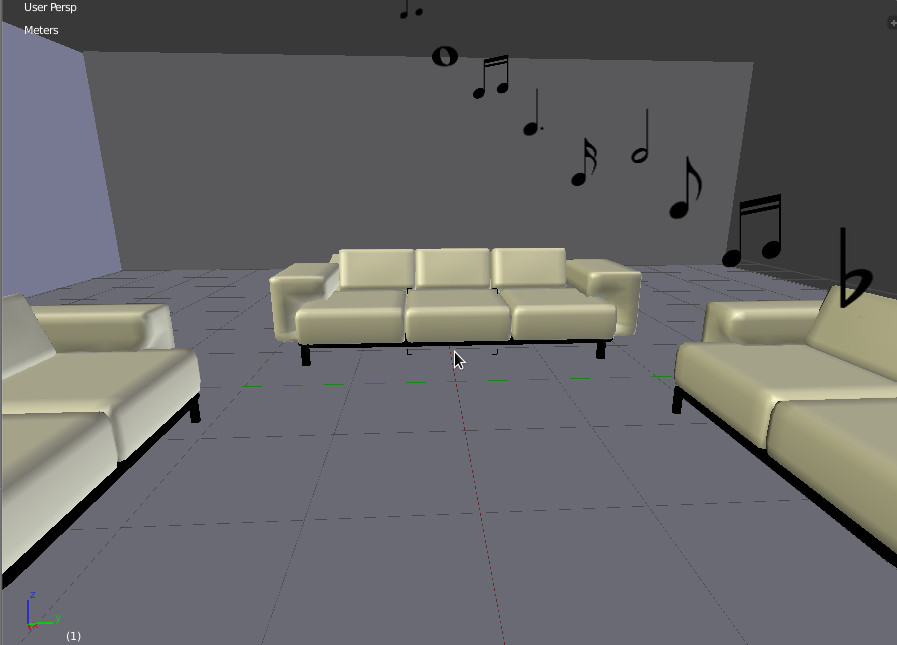
\includegraphics[width=90mm]{images/design/GD_basic.jpg}
\caption{Room with one object generating sound}
\label{sensorymockup1}
\end{figure}

\begin{figure}[H]
\centering
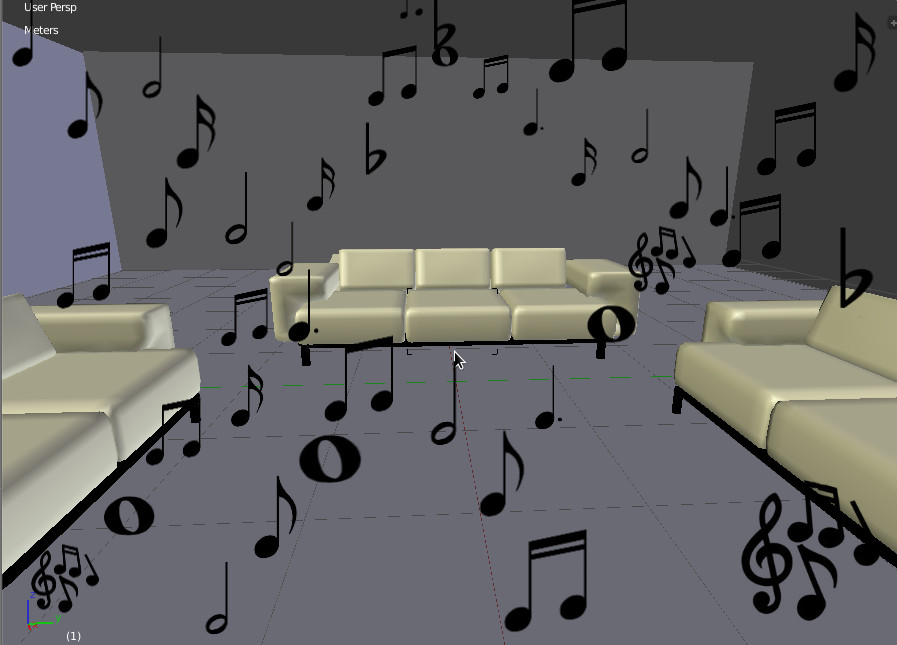
\includegraphics[width=90mm]{images/design/GD_moresound.jpg}
\caption{Effects of multiple objects creating sound}
\label{sensorymockup2}
\end{figure}

\begin{figure}[H]
\centering

\includegraphics[width=90mm]{images/design/GD_overload.jpg}
\caption{Sensory overload. Lights have become brighter and environment is harder to see. Gaussian filter applied}
\label{sensorymockup3}
\end{figure}

\section{Results}
Interviews were an invaluable contribution to the project that gave insight and feedback into the Autism world currently not found from literature. As interviews were guided by the interviewee, some interesting and finding were observed. In addition, obtaining information from a teacher with large amount of experience in the domain revealed problems when new trainee teachers arrived and how they interacted with children with autism in class.  

Sensory difficulties was particularly prominent for two interviews "I was just so traumatised by the time I got to school with all these different noises, smells in the car and overload of sensory information. I'd just sit in silence and I couldn’t explain to anyone around me what was going on. When I finally arrived home, it just all came out as anger, rage even and my parents never knew why."[C3]. "The noises in the playground were just too much. So i'd sit by the edge of the playground and watch cars go past because those at least were predictable. I used to do this with slinkys on the stairs as well. The sound was beautiful."[C3]. [C4] also specified that for them to replenish energy a quiet environment was required and that "special interests" could be "literally used to replenish energy levels". [C4] in addition specified that as a child they would take coins around with them everywhere they went so they can spin them and use this to alleviate some of the turbulant sensory experiences "I used to do this in school and teachers didn't like that I wasn't paying attention to them. They didn't know that playing with them actually helped me to focus on what they were saying".

[C3] specified they were unable to communicate difficulties until much older however this is contrasted with another interview that felt "I'm pretty good at verbalising my problems, I've always been quite good at doing so although people don't always understand" [C5]. Although the prevalent theme of wanting more understanding was apparent, it was interesting to see the differences in obstacles faced and highlights the need for the simulator to be flexible. 

Changes in routine and structure were also highlighted a predominant cause of stress and anxiety as "A good day would be a structured day with no unpredictable events or changes in routine. Changes in routine can really make me anxious. And when I don't wake up with anxiety, sometimes anxiety can last for days. Also, if the weather is nice, that can help a good day" [C5]

The hardest difficulties highlighted by both teachers was "Language, communication and information processing delay. "A lot of staff have verbal diarrhoea and we have to keep reminding them to give black and white information or time to answer questions. Also the delayed processing of information where staff keep repeatedly asking questions without giving them time to think."[C2] and such events were said to sometimes lead to a meltdown. [C2] also spoke of the difficulty with contrasting sensory needs in the classroom, if a child required visual simulation which manifested as turning the lights on and off it could cause sensory issues for another child whom is sensitive. 


\section{Conclusions: Goals and restrictions identified}

2 of the 3 people interviewed specified that found the images of the sensory overloads extremely uncomfortable to view(and quickly looked away), and that it was an accurate representation. This demonstrated that a sensory overload differs for each individual and indicates more should be consulted as 3 is a small sample. However, the projects core aim is to raise awareness of these problems rather than attempting to give an identical experience of having autism and thus the mock images will be used unless feedback in the formative evaluation indicates changes are required. 

From the interviews conducted, the choice of project was solidified as well as the difficulties chosen to convey:

\begin{enumerate}
\item Sensory atypicalities: selected as the primary difficulty to convey due to their prevalence and hidden nature which is less known to the public
\item Meltdowns: As these can be caused by sensory atypicalities and it is important to convey to the user the impact of difficulties, not just the difficulties themselves.
\item Special interests: A means in the game to 'soothe' the character and counteract meltdowns.
\item Information processing delays: commented as a big problem in the classroom.
\end{enumerate}

Due to the complexity of conveying social and communication problems it was decided not to include this in the first version despite its prevalence in autism life. Sensory processing problems were selected as as this was a prominent theme in interviews and listening to individuals speaking of the trauma, the inability to communicate and seek help was really heart-felt. Information processing was selected as teachers highlighted this as a main cause to meltdowns in the classroom. 